\begin{figure}[htbp]
\centering
\begin{tabular}{@{}c@{\hspace{10mm}}c@{}}
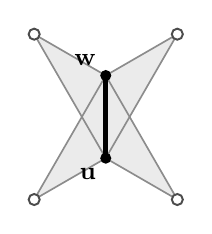
\begin{tikzpicture}[baseline]
  \fill[black!8] (0.000,0.000) -- (-0.909,-0.525) -- (0.000,1.050) -- cycle;
  \fill[black!8] (0.000,0.000) -- (-0.909,1.575) -- (0.000,1.050) -- cycle;
  \fill[black!8] (0.000,0.000) -- (0.909,-0.525) -- (0.000,1.050) -- cycle;
  \fill[black!8] (0.000,0.000) -- (0.909,1.575) -- (0.000,1.050) -- cycle;
  \draw[black!45,line width=0.6pt] (0.000,0.000) -- (-0.909,-0.525) -- (0.000,1.050);
  \draw[black!45,line width=0.6pt] (0.000,0.000) -- (-0.909,1.575) -- (0.000,1.050);
  \draw[black!45,line width=0.6pt] (0.000,0.000) -- (0.909,-0.525) -- (0.000,1.050);
  \draw[black!45,line width=0.6pt] (0.000,0.000) -- (0.909,1.575) -- (0.000,1.050);
  \draw[line width=1.8pt,black] (0.000,0.000) -- (0.000,1.050);
  \fill[white] (-0.909,-0.525) circle (2.0pt); \draw[black!70,line width=0.7pt] (-0.909,-0.525) circle (2.0pt);
  \fill[white] (-0.909,1.575) circle (2.0pt); \draw[black!70,line width=0.7pt] (-0.909,1.575) circle (2.0pt);
  \fill[white] (0.909,-0.525) circle (2.0pt); \draw[black!70,line width=0.7pt] (0.909,-0.525) circle (2.0pt);
  \fill[white] (0.909,1.575) circle (2.0pt); \draw[black!70,line width=0.7pt] (0.909,1.575) circle (2.0pt);
  \fill[black] (0.000,0.000) circle (2.0pt); \fill[black] (0.000,1.050) circle (2.0pt);
  \node[anchor=north east,font=\small] at (0.000,0.000) {$\mathbf u$};
  \node[anchor=south east,font=\small] at (0.000,1.050) {$\mathbf w$};
\end{tikzpicture}
&
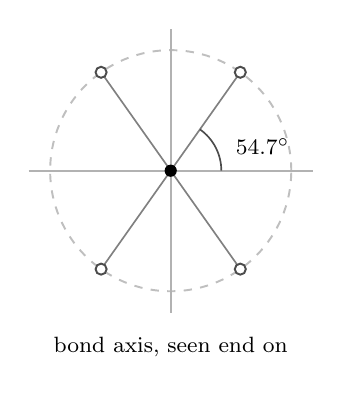
\begin{tikzpicture}[baseline]
  \draw[black!25,dashed,line width=0.7pt] (0,0) circle (1.531);
  \draw[black!30,line width=0.6pt] (-1.806,0) -- (1.806,0);
  \draw[black!30,line width=0.6pt] (0,-1.806) -- (0,1.806);
  \draw[black!50,line width=0.6pt] (0,0) -- (-0.884,-1.250);
  \fill[white] (-0.884,-1.250) circle (2.0pt); \draw[black!70,line width=0.7pt] (-0.884,-1.250) circle (2.0pt);
  \draw[black!50,line width=0.6pt] (0,0) -- (-0.884,1.250);
  \fill[white] (-0.884,1.250) circle (2.0pt); \draw[black!70,line width=0.7pt] (-0.884,1.250) circle (2.0pt);
  \draw[black!50,line width=0.6pt] (0,0) -- (0.884,-1.250);
  \fill[white] (0.884,-1.250) circle (2.0pt); \draw[black!70,line width=0.7pt] (0.884,-1.250) circle (2.0pt);
  \draw[black!50,line width=0.6pt] (0,0) -- (0.884,1.250);
  \fill[white] (0.884,1.250) circle (2.0pt); \draw[black!70,line width=0.7pt] (0.884,1.250) circle (2.0pt);
  \fill[black] (0,0) circle (2.2pt);
  \draw[black!70,line width=0.6pt] (0.643,0) arc (0:54.74:0.643);
  \node[font=\footnotesize,anchor=west] at (0.704,0.306) {$54.7^\circ$};
  \node[font=\footnotesize,anchor=north] at (0,-1.990) {bond axis, seen end on};
\end{tikzpicture}
\\[1mm]
{\footnotesize (a) the four triangles on a bond} & {\footnotesize (b) the same four, seen along the bond} \\
\end{tabular}
\caption{Illustration of an apex. (a) Every edge bond belongs to exactly four triangles, and they are
equilateral: each apex is $\sqrt2\,h$ from both ends, the same distance the two ends are from each
other.
(b) Looking along the bond. All four apexes lie in its perpendicular bisector plane at the same
distance from the axis, so they sit on a circle.}
\label{fig:si-apex}
\end{figure}
